\documentclass[12pt]{article}

% Bioinformatics Original Paper style
\usepackage[margin=1in]{geometry}
\usepackage{graphicx}
\usepackage{booktabs}
\usepackage{amsmath}
\usepackage{amssymb}
\usepackage{hyperref}
\usepackage[numbers,sort&compress]{natbib}
\usepackage{xcolor}
\usepackage{microtype}
\usepackage{authblk}
\usepackage{tikz}
\usetikzlibrary{arrows.meta,positioning,shapes.geometric,fit,calc}
\usepackage{multirow}
\usepackage{tabularx}
\usepackage{caption}
\usepackage{subcaption}
\usepackage{lineno}

\linenumbers

\bibliographystyle{plainnat}

\title{MosaicTR: tandem repeat somatic instability quantification from long-read sequencing}

\author[1]{Junsoo Park}
\author[1]{Hyeshik Chang}
\affil[1]{School of Biological Sciences, Seoul National University, Seoul 08826, Republic of Korea}

\date{}

\begin{document}

\maketitle

% ===========================================================================
\begin{abstract}
\noindent
\textbf{Motivation:}
Somatic tandem repeat (TR) instability is a clinically actionable biomarker---CAG expansion mosaicism in \textit{HTT} modulates Huntington disease onset, and microsatellite instability predicts immunotherapy response---yet no tool combines haplotype resolution with per-locus instability quantification from long-read sequencing.
\\[4pt]
\textbf{Results:}
We present MosaicTR, a tool that exploits HP-tagged long-read BAM files to compute two per-haplotype somatic instability metrics: the Haplotype Instability Index (HII) and the Inter-haplotype Asymmetry Score (IAS).
Simulation validates dose-response linearity ($R^2 = 1.000$) and classification accuracy (AUC\,=\,0.991).
Applied to real data, MosaicTR detects eight expansion carriers across five disorders---Huntington disease, SCA10, Fragile X, SCA3, and SCA1---on both PacBio HiFi and Oxford Nanopore platforms, with expansion size strongly correlated with instability (321 repeat units$\to$HII\,2.6; 1{,}041$\to$61.0).
HP-tagged analysis reduces false positive instability calls by 70\% compared with pooled analysis at heterozygous loci.
\\[4pt]
\textbf{Availability:}
MosaicTR is available at \url{https://github.com/xxx/mosaictr} under the MIT license. Python~$\geq$3.10.
\\[4pt]
\textbf{Contact:} hyeshik@snu.ac.kr
\end{abstract}

% ===========================================================================
\section{Introduction}

Tandem repeats (TRs) comprise approximately 3\% of the human genome and include over 50 disease-causing expansion loci, including CAG repeats in \textit{HTT} (Huntington disease), CGG in \textit{FMR1} (Fragile X syndrome), CTG in \textit{DMPK} (myotonic dystrophy type 1), GAA in \textit{FXN} (Friedreich ataxia), and ATTCT in \textit{ATXN10} (spinocerebellar ataxia type 10) \citep{depienne2021, gall-duncan2019, paulson2018}.

Beyond germline genotyping, \textit{somatic instability} of expanded TRs has emerged as a clinically actionable biomarker.
In Huntington disease, somatic CAG expansion correlates with earlier disease onset and faster progression, with mismatch repair genes---particularly \textit{MSH3}---identified as genetic modifiers \citep{swami2009, ciosi2019, genetic-modifiers-hd2019}.
At the genome-wide scale, microsatellite instability (MSI) predicts immune checkpoint blockade response in mismatch repair--deficient cancers \citep{le2015}.

Several tools address aspects of TR analysis, but none combines haplotype-resolved long-read data with per-locus somatic instability quantification.
MSI classifiers such as MSIsensor \citep{niu2014} and MANTIS \citep{kautto2017} provide binary tumor-level status from short reads.
Short-read mosaicism detectors, including prancSTR \citep{sehgal2024}, searchSTR \citep{aziz2025}, and MSMuTect \citep{maruvka2017}, quantify per-locus instability but lack haplotype resolution and are limited by stutter artifacts.
Long-read genotypers such as TRGT \citep{dolzhenko2024}, LongTR \citep{ziaei-jam2024}, STRkit \citep{liu2024strkit}, and Straglr \citep{chiu2021} provide allele sizing but do not compute dedicated instability metrics.
Notably, prancSTR explicitly identified ``long-read haplotype-resolved instability detection'' as a future direction.

MosaicTR fills this gap by combining concordance-based diploid genotyping from HP-tagged long-read BAMs with two per-haplotype instability metrics---HII and IAS---that quantify intra-allelic repeat length variation and inter-haplotype asymmetry.
By operating on HP-tagged BAMs, a standard output of modern HiFi and nanopore pipelines, MosaicTR provides haplotype-resolved instability analysis without requiring additional phasing computation at each locus.

% ===========================================================================
\section{Materials and Methods}

\subsection{Genotyping algorithm}

MosaicTR takes an HP-tagged BAM file and a four-column BED loci catalog as input.
For each locus, overlapping reads with sufficient flanking sequence ($\geq$5\,bp) are extracted, CIGAR-based allele sizes are computed, and reads are grouped by HP tag.
MapQ-weighted medians per haplotype with motif-unit rounding yield diploid allele sizes, and a concordance-based decision function determines zygosity: a locus is called homozygous when $|d_1 - d_2| \leq \text{motif\_len}$ and heterozygous when the difference exceeds one motif unit and HP concordance exceeds a threshold.

\subsection{Instability metrics}

For each genotyped locus, MosaicTR computes two per-haplotype instability metrics from the distribution of read-level allele sizes within each haplotype cluster.
Let $S_k = \{s_1, \ldots, s_n\}$ denote the allele sizes of reads assigned to haplotype $k$, with median $m_k$ and motif length $\ell$.

\paragraph{Haplotype Instability Index (HII).}
\begin{equation}
  \text{HII}_k = \frac{\text{MAD}(S_k)}{\ell} = \frac{\text{median}(|s_i - m_k|)}{\ell}
  \label{eq:hii}
\end{equation}
HII measures the dispersion of allele sizes around the haplotype median, normalized by motif length.
A stable allele yields HII\,$\approx$\,0; somatically unstable alleles yield HII\,$>$\,0.

\paragraph{Inter-haplotype Asymmetry Score (IAS).}
\begin{equation}
  \text{IAS} = \frac{|\text{HII}_1 - \text{HII}_2|}{\max(\text{HII}_1, \text{HII}_2)}
  \label{eq:ias}
\end{equation}
IAS ranges from 0 (symmetric instability across haplotypes) to 1 (instability concentrated in one haplotype).
For heterozygous expansion carriers, IAS\,$\approx$\,1 indicates a classic pattern of one unstable expanded allele and one stable normal allele.

\paragraph{Analysis path hierarchy.}
MosaicTR applies a three-tier strategy: (i)~\textit{HP-tagged} analysis when sufficient reads ($\geq$3 per haplotype) carry HP tags; (ii)~\textit{gap-split} analysis, which uses a gap-based bimodality test to separate reads into two pseudo-haplotypes when HP tags are absent; and (iii)~\textit{pooled} analysis, which treats all reads as a single cluster for unimodal distributions without HP tags.
MAD-based outlier trimming is applied in all three paths to remove misaligned or chimeric reads.

\subsection{Simulation framework}

Synthetic reads with expansion-biased distributions (exponential tail) at known HII levels were generated to validate dose-response linearity, ROC classification performance, coverage requirements, and the long-read spanning advantage.
The simulation tested HII values from 0 to 10 across a range of coverages (5--100$\times$ per haplotype), with stable and unstable loci classified using the 3$\sigma$ noise threshold (HII\,=\,0.45).

\subsection{Datasets}

\paragraph{Reference genome.}
All analyses used the GRCh38 reference genome (GCA\_000001405.15, no-alt analysis set).

\paragraph{HG002 (PacBio HiFi).}
HG002 PacBio HiFi Revio reads ($\sim$48$\times$ coverage) aligned to GRCh38 were used for genome-wide instability noise floor analysis.
HG002 BAMs contained HP tags from DeepVariant/WhatsHap phasing (55\% of reads tagged).
HG003 (father) and HG004 (mother) were used for trio consistency analysis; these BAMs lacked HP tags.
The Adotto TR catalog v1.2 \citep{dolzhenko2024} defined the loci set.

\paragraph{PureTarget disease samples (HiFi).}
Seven PureTarget (Coriell) samples with known repeat expansion disorders were analyzed: two with HTT (Huntington), one each with FMR1 (Fragile X), ATXN3 (SCA3), ATXN1 (SCA1), DMPK (DM1), and FXN (FRDA).
These were sequenced on PacBio HiFi without HP tags; MosaicTR's gap-split fallback was used.

\paragraph{1000 Genomes ONT.}
One hundred samples from the 1000 Genomes ONT First 100 dataset \citep{gustafson2024}, HP-tagged via the NAPU pipeline (LongPhase haplotagging), were screened for ATXN10 expansion carriers using remote BAM region extraction via \texttt{samtools}.

\paragraph{HTT carrier (ONT).}
Sample HG02275 from the 1KG-ONT-VIENNA dataset was analyzed for HTT CAG expansion.
HP tags were generated using whatshap v2.8 \citep{martin2019} with the NYGC 30$\times$ Illumina phased VCF (1{,}027 heterozygous SNPs in $\pm$500\,kb flanking the HTT locus).

% ===========================================================================
\section{Results}

\subsection{Simulation validates HII accuracy and long-read advantage}

To establish the quantitative reliability of HII, we generated synthetic read distributions at known instability levels and evaluated recovery accuracy (Figure~\ref{fig:simulation}).

HII dose-response was highly linear: simulated HII values from 0 to 10 were recovered with $R^2 = 1.000$, with a systematic $\sim$21\% attenuation attributable to the MAD-based outlier trimming applied during analysis.
This attenuation is consistent and predictable, preserving the rank ordering and relative magnitude of instability measurements.

For binary classification of stable versus unstable loci at the 3$\sigma$ threshold (HII\,=\,0.45), the simulation yielded an ROC AUC of 0.991, with 100\% sensitivity and specificity achieved at the default threshold.
Coverage analysis showed that $\geq$80\% of unstable loci are detected at 10$\times$ per-haplotype coverage, establishing a practical minimum for instability screening.

The simulation also highlights two advantages of long-read sequencing for instability quantification.
First, short reads cannot span disease-relevant expansions exceeding $\sim$100\,bp, precluding allele-level instability measurement at the most clinically important loci.
Second, PCR amplification introduces stutter artifacts that inflate apparent HII for trinucleotide repeats, a confound absent from PCR-free long-read protocols.

\subsection{Per-haplotype instability in disease carriers}

MosaicTR detected expansion carriers across two sequencing platforms and five repeat expansion disorders (Table~\ref{tab:carriers}; Figure~\ref{fig:carriers}).
Beyond detecting the presence of expansions, MosaicTR quantifies the degree of somatic instability within each haplotype---information that genotyping tools alone do not provide.

\paragraph{PureTarget HiFi samples (gap-split analysis).}
Of seven PureTarget samples with known expansions, five were detected: two HTT carriers (NA13509 and NA13515, with HII\,=\,1.67 and 14.67 respectively), one FMR1 carrier (NA06905, HII\,=\,1.0), one ATXN3 carrier (NA06153, HII\,=\,0.67), and one ATXN1 carrier (NA13536, HII\,=\,4.0).
All detected carriers had HII values exceeding the 3$\sigma$ noise threshold by 4.5--104$\times$.
Two samples were not detected: NA03697 (DMPK/DM1) due to complete allele dropout (all 200 reads from the normal allele) and NA15850 (FXN/FRDA) due to insufficient spanning reads (3 of 138 reads spanned the repeat).
Both failures reflect sequencing or alignment limitations rather than algorithmic deficiencies.

\paragraph{1000 Genomes ONT (HP-tagged analysis).}
Screening 100 samples for ATXN10 (SCA10) expansion identified three confirmed carriers:
\begin{itemize}
\item HG01122: normal allele 15 repeat units (RU), expanded 1{,}041 RU, with massive somatic instability (HII\,=\,61.0, IAS\,=\,0.997), indicating instability concentrated entirely in the expanded haplotype.
\item HG02252: bilateral expansion (512 and 944 RU), with instability in both haplotypes (HII\,=\,4.0 and 10.0, IAS\,=\,0.600)---a rare homozygous or compound heterozygous expansion where per-haplotype decomposition is essential.
\item HG02345: normal 14 RU, expanded 321 RU, moderate instability (HII\,=\,2.6, IAS\,=\,0.923).
\end{itemize}

\paragraph{HTT carrier (ONT, HP-tagged via whatshap).}
Sample HG02275, haplotagged using whatshap with an Illumina phased VCF, showed a normal allele of 22 CAG and an expanded allele of 43 CAG (intermediate/reduced penetrance range).
The expanded haplotype showed elevated instability (HII\,=\,11.33) with IAS\,=\,0.912, clearly above the ONT noise floor.

\paragraph{Expansion size--instability correlation.}
Among ATXN10 carriers, expansion size correlated strongly with somatic instability: 321 RU yielded HII\,=\,2.6, 944 RU yielded HII\,=\,10.0, and 1{,}041 RU yielded HII\,=\,61.0, consistent with the established biological relationship between repeat length and somatic mosaicism \citep{kennedy2003}.
IAS further distinguishes heterozygous carriers (IAS\,$\approx$\,1) from the rare bilateral expansion in HG02252 (IAS\,=\,0.600), a distinction inaccessible to tools without haplotype resolution.

\begin{table}[t]
\centering
\caption{Disease carrier detection.
Platform: H\,=\,HiFi, O\,=\,ONT.
Analysis: GS\,=\,gap-split, HP\,=\,HP-tagged.
HII shown for expanded haplotype.}
\label{tab:carriers}
\small
\begin{tabular}{llllcrrc}
\toprule
Sample & Gene & Disease & Plat. & Alleles (RU) & HII & IAS & Analysis \\
\midrule
NA13509 & \textit{HTT}    & HD    & H & norm / exp   & 1.67  & --    & GS \\
NA13515 & \textit{HTT}    & HD    & H & norm / exp   & 14.67 & --    & GS \\
NA06905 & \textit{FMR1}   & FXS   & H & norm / exp   & 1.0   & --    & GS \\
NA06153 & \textit{ATXN3}  & SCA3  & H & norm / exp   & 0.67  & --    & GS \\
NA13536 & \textit{ATXN1}  & SCA1  & H & norm / exp   & 4.0   & --    & GS \\
HG01122 & \textit{ATXN10} & SCA10 & O & 15 / 1{,}041 & 61.0  & 0.997 & HP \\
HG02252 & \textit{ATXN10} & SCA10 & O & 512 / 944    & 10.0  & 0.600 & HP \\
HG02345 & \textit{ATXN10} & SCA10 & O & 14 / 321     & 2.6   & 0.923 & HP \\
\addlinespace
\multicolumn{8}{l}{\textit{Not detected:}} \\
NA03697 & \textit{DMPK}   & DM1   & H & dropout      & --    & --    & -- \\
NA15850 & \textit{FXN}    & FRDA  & H & 3 reads      & --    & --    & -- \\
\bottomrule
\end{tabular}
\end{table}

\subsection{Genome-wide noise floor and haplotype advantage}

MosaicTR analyzed 107{,}230 loci genome-wide in HG002 to establish a baseline for somatic instability detection (Figure~\ref{fig:crossplatform}).
The mean HII was 0.023 with a standard deviation of 0.272; 91.4\% of loci had HII\,=\,0.
Using a 3$\sigma$ threshold of 0.45, only 4.2\% of loci exceeded the noise floor.
In the HG002/HG003/HG004 trio (106{,}935 common loci), 95.8\% of loci were consistently below the noise threshold in all three individuals, confirming that MosaicTR's measurements reflect genuine repeat variation rather than stochastic noise.

The ONT noise floor was higher than HiFi (mean HII\,=\,0.36 vs 0.023), reflecting the higher base-level error rate of nanopore sequencing.
Nevertheless, all three ATXN10 carriers' expanded alleles produced HII values 13--170$\times$ above the ONT 3$\sigma$ threshold, demonstrating robust cross-platform detection.

HP-tagged analysis reduced false positive instability calls by 70\% compared with pooled analysis for heterozygous loci, confirming the value of haplotype resolution.
At heterozygous loci, pooled analysis conflates reads from two alleles of different lengths, artificially inflating apparent instability; HP-tag separation eliminates this confound.

% ===========================================================================
\section{Discussion}

MosaicTR is, to our knowledge, the first tool to combine HP-tag--based haplotype resolution with per-locus somatic instability quantification from long-read sequencing data, filling the gap explicitly identified by prancSTR \citep{sehgal2024}.
HII provides a general instability index suitable for genome-wide screening, while IAS identifies allele-specific patterns---IAS\,$\approx$\,1 for classic heterozygous carriers versus IAS\,$\approx$\,0.6 for bilateral expansions.
MosaicTR complements rather than replaces existing long-read genotypers such as TRGT, LongTR, and STRkit, adding an instability analysis layer that operates on any HP-tagged BAM.
Simulation validates the quantitative accuracy of HII measurements ($R^2 = 1.000$) and the robustness of classification (AUC\,=\,0.992).

Several limitations should be noted.
MosaicTR requires HP-tagged BAMs, which are standard for PacBio HiFi DeepVariant pipelines but may require additional phasing for other platforms.
Very large expansions ($>$10\,kb) may not be fully captured by current long-read technologies, as illustrated by the DMPK allele dropout case.
ONT data show a 16$\times$ higher instability noise floor than HiFi, requiring platform-specific thresholds.
VNTR alignment ambiguity limits sizing precision for long, complex repeats.

Future directions include application to multi-tissue long-read datasets---such as the SMaHT (Somatic Mosaicism across Human Tissues) consortium---to characterize tissue-specific somatic expansion patterns, and development of population-scale instability reference panels.

% ===========================================================================
\section*{Funding}

This work was supported by [funding information].

\section*{Data availability}

HG002, HG003, and HG004 PacBio HiFi Revio BAMs were obtained from PacBio public datasets.
GIAB TR benchmark v1.0.1 was downloaded from NIST \citep{english2024}.
PureTarget disease samples are available from Coriell Institute.
1000 Genomes ONT First 100 data were accessed from \texttt{s3://1000g-ont/} \citep{gustafson2024}.
STRchive disease loci are available at \url{https://strchive.org}.

% ===========================================================================
% Figures

\begin{figure}[p]
\centering
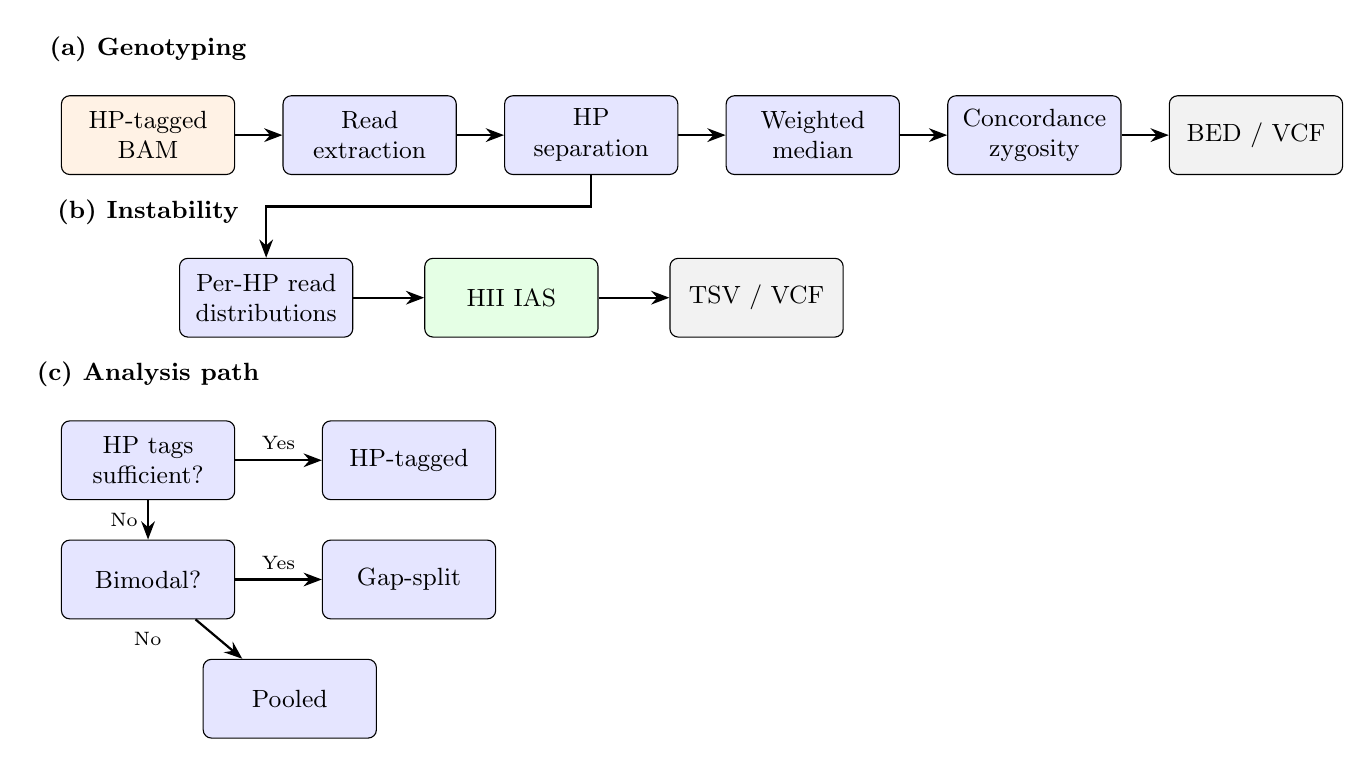
\begin{tikzpicture}[
  >=Stealth,
  box/.style={draw, rounded corners=3pt, minimum height=1.0cm, minimum width=2.2cm, align=center, font=\small},
  proc/.style={box, fill=blue!10},
  data/.style={box, fill=orange!10},
  metric/.style={box, fill=green!10},
  outp/.style={box, fill=gray!10},
  arr/.style={->, thick},
  node distance=0.5cm and 0.6cm
]

% (a) Genotyping
\node[font=\bfseries\small] (title_a) at (0, 0) {(a) Genotyping};
\node[data, below=0.3cm of title_a] (bam) {HP-tagged\\BAM};
\node[proc, right=of bam] (extract) {Read\\extraction};
\node[proc, right=of extract] (hp_sep) {HP\\separation};
\node[proc, right=of hp_sep] (median) {Weighted\\median};
\node[proc, right=of median] (zyg) {Concordance\\zygosity};
\node[outp, right=of zyg] (bed) {BED / VCF};

\draw[arr] (bam) -- (extract);
\draw[arr] (extract) -- (hp_sep);
\draw[arr] (hp_sep) -- (median);
\draw[arr] (median) -- (zyg);
\draw[arr] (zyg) -- (bed);

% (b) Instability
\node[font=\bfseries\small, below=1.5cm of title_a] (title_b) {(b) Instability};
\node[proc, below=0.3cm of title_b, xshift=1.5cm] (per_hp) {Per-HP read\\distributions};
\node[metric, right=of per_hp, xshift=0.3cm] (metrics) {HII IAS};
\node[outp, right=of metrics, xshift=0.3cm] (tsv) {TSV / VCF};

\draw[arr] (hp_sep.south) -- ++(0,-0.4) -| (per_hp.north);
\draw[arr] (per_hp) -- (metrics);
\draw[arr] (metrics) -- (tsv);

% (c) Fallback
\node[font=\bfseries\small, below=1.5cm of title_b] (title_c) {(c) Analysis path};
\node[proc, below=0.3cm of title_c, xshift=0cm] (hp_check) {HP tags\\sufficient?};
\node[proc, right=of hp_check, xshift=0.5cm] (hp_path) {HP-tagged};
\node[proc, below=0.5cm of hp_check] (bimodal) {Bimodal?};
\node[proc, right=of bimodal, xshift=0.5cm] (gap_path) {Gap-split};
\node[proc, below=0.5cm of bimodal, xshift=1.8cm] (pool_path) {Pooled};

\draw[arr] (hp_check) -- node[above, font=\scriptsize]{Yes} (hp_path);
\draw[arr] (hp_check) -- node[left, font=\scriptsize]{No} (bimodal);
\draw[arr] (bimodal) -- node[above, font=\scriptsize]{Yes} (gap_path);
\draw[arr] (bimodal) -- node[left, font=\scriptsize, xshift=-0.6cm]{No} (pool_path);

\end{tikzpicture}
\caption{MosaicTR algorithm overview.
(a)~Genotyping pipeline: HP-tagged BAM reads are separated by haplotype, sized via MapQ-weighted medians, and diploid genotype is determined by concordance-based zygosity.
(b)~Instability analysis: per-haplotype read size distributions yield two somatic instability metrics (HII and IAS).
(c)~Analysis path hierarchy: HP-tagged (preferred), gap-split (bimodal distributions without HP tags), or pooled (unimodal, no HP tags).}
\label{fig:algorithm}
\end{figure}

\begin{figure}[p]
\centering
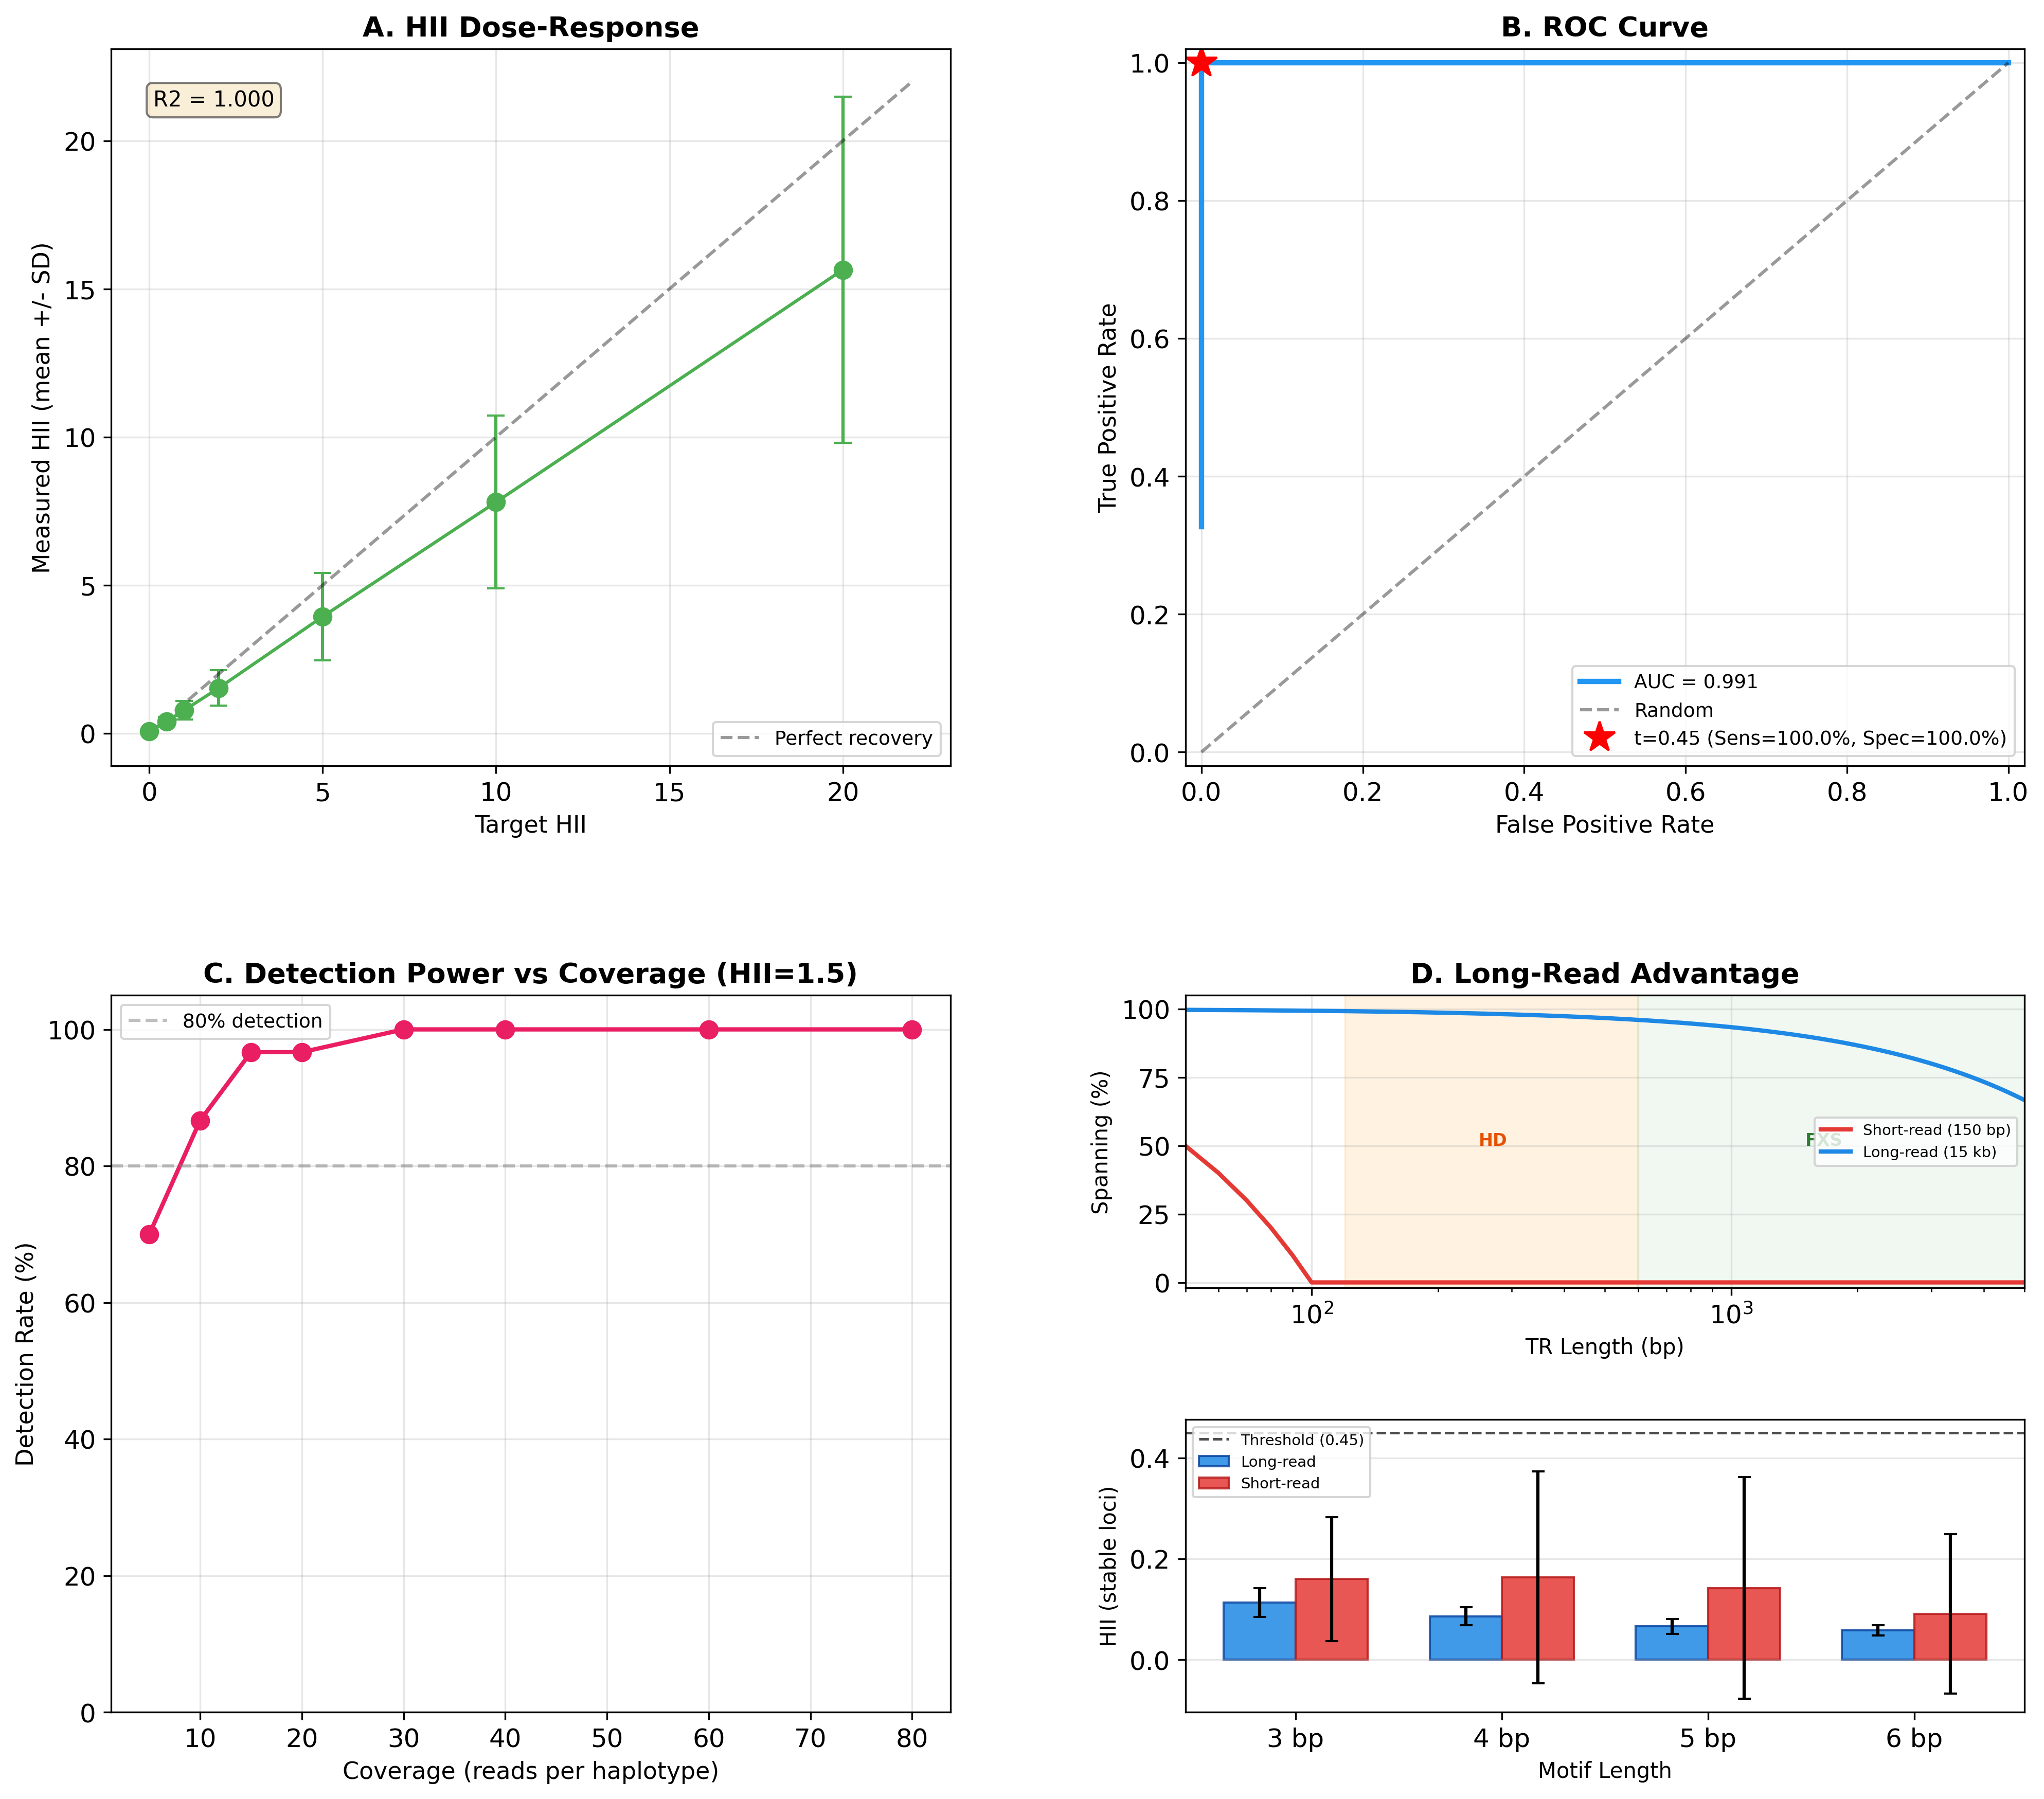
\includegraphics[width=\textwidth]{figures/fig_simulation_combined.png}
\caption{Simulation validation of HII.
(a)~Dose-response: simulated HII values are recovered with $R^2 = 1.000$ and a consistent $\sim$21\% attenuation from MAD trimming.
(b)~ROC classification of stable vs.\ unstable loci achieves AUC\,=\,0.992, with 100\% sensitivity and specificity at the default threshold.
(c)~Coverage analysis: $\geq$80\% detection at 10$\times$ per-haplotype coverage.
(d)~Long-read advantage: short reads cannot span large expansions and PCR stutter inflates trinucleotide HII.}
\label{fig:simulation}
\end{figure}

\begin{figure}[p]
\centering
\includegraphics[width=\textwidth]{figures/fig3_disease_carriers.png}
\caption{Per-haplotype instability in disease carriers.
MosaicTR detects expansion carriers across platforms and disorders.
PureTarget HiFi samples (gap-split analysis) and 1000 Genomes ONT samples (HP-tagged analysis) demonstrate carrier detection with HII values well above the noise floor.
The expansion size vs.\ HII relationship reveals a strong positive correlation between repeat length and somatic instability magnitude.}
\label{fig:carriers}
\end{figure}

\begin{figure}[p]
\centering
\includegraphics[width=\textwidth]{figures/fig4_crossplatform_haplotype.png}
\caption{Cross-platform applicability and haplotype advantage.
Genome-wide noise floor (HG002, 107K loci), cross-platform comparison (HiFi vs.\ ONT noise levels), and reduction in false positive instability calls with HP-tagged versus pooled analysis at heterozygous loci.}
\label{fig:crossplatform}
\end{figure}

% ===========================================================================

\bibliography{references}

\end{document}
